\newpage
\subsection{Editing device layers}
\label{sec:layereditor}

\begin{minipage}{0.5\textwidth}
\centering
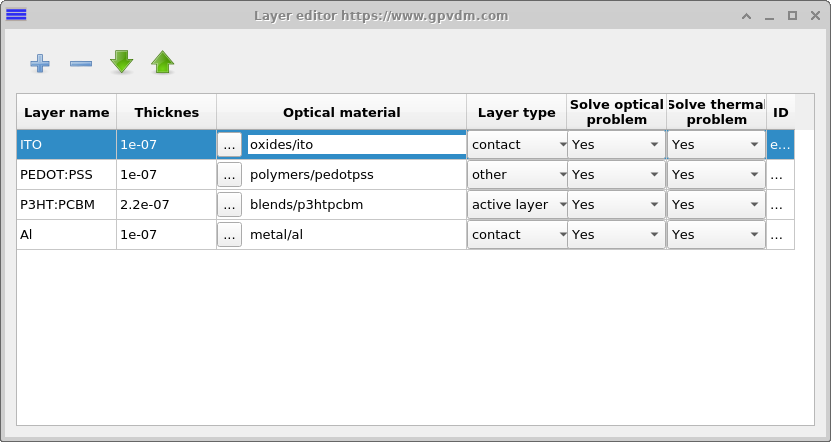
\includegraphics[width=\textwidth,height=0.7\textwidth]{./images/running/layer_editor.png}
\captionof{figure}{The layer editor window.}
\label{fig:layereditor}
\end{minipage}
\begin{minipage}[]{0.5\linewidth}
\hspace*{8px}
Any device in OghmaNano consists of a series of layers (this is sometimes referred to as the epitaxy - this is a term which comes from inorganic semiconductors). The layer editor can be accessed from the main simulation window, under the \emph{device structure} tab. This is visible towards the top of figure \ref{fig:simpleinterface}, and the layer editor is visible in figure \ref{fig:layereditor}. Within the window is a table that describes the structure of the device. The column thickness describes the thickness of each layer. The P3HT:PCBM layer is the layer of material which converts photons into electrons and holes, this is commonly called the active layer.
\end{minipage}
\vspace*{8px}
 An active layer thickness of 50nm is considered very thin for an organic solar cell, while an active layer of 400nm is considered very thick (too thick for efficient device operation). Vary the active layer between 50 nm and 400 nm, for each thickness record the device efficiency (I suggest you perform the simulation for at least eight active layer widths).



\subsubsection{More on the layer editor}
The layer editor has the following columns:

\begin{itemize}
  \item Layer name: Is the English name describing the layer. You can call your layers what you want (i.e. ITO, PEDOT, fred or bob) it has no physical meaning.
  \item Thickness: Is the layer thickness given in meters.
  \item Optical material: Specifies the n/k data which is used to describe the materials optical properties. In the simulation the n/k data are taken from experimental values stored in the optical database \ref{sec:materialdatabase} and have nothing to do with the electrical material properties such as effective band gap.
  \item Layer type: Specifies to the simulation how the layer is treated when performing a simulation. There are three types of layer
	\begin{itemize}
	  \item active: This type of layer is electrically active and the drift diffusion solver will solve the electrical equations in this layer type. See section \ref{sec:electrical}. You can have as many active layers as you like but they must be contiguous.
 	  \item contact: This tells the model that a layer is a contact and a voltage should be applied, see section \ref{sec:contacteditor} for more details.
 	  \item other: Any layer which is not a contact or active.

	\end{itemize}
\end{itemize}

%\vspace*{\fill}


\subsubsection{Which layers should be active?}
A common mistake people make when starting to simulate devices is to try to make all the layers in their device active because their logic is: Current must be flowing through them so they must be active right?  However, in for example a solar cell only the BHJ or in a perovskite device the perovskite layer will have both species of carriers (electrons+holes) and complex effects such as photogeneration, recombination and carrier trapping. So in this layer it makes sense to solver the drift diffusion equations.  Other layers which don't have both species of carriers can be treated simple parasitic resistances see section \ref{sec:parasitic}. I would only recommend setting other layers of the device to active (such as the HTL/ETL) if you are trying to investigate effects such as s-shaped JV curves or devices which clearly need multiple active layers such as OLEDs. In general, try to minimize the number of active layers and always keep simulations as simple as possible to explain the physical effects you see.  

\vspace*{\fill}
\fbox{
\parbox{0.9\textwidth}{
\color{blue} Task \addtocounter{question}{1}\thequestion : Plot a graph (using excel or any other graphing tool), of device efficiency v.s. thickness of the active layer. What is the optimum efficiency/thickness of the active layer? Also plot graph $V_{oc}$ , $J_{sc}$ and $FF$
as a function of active layer thickness. $J_{sc}$ is generally speaking the maximum current a solar cell can generate, try to explain your graph of J sc
v.s. thickness, [Hint, the next section may help you answer this part of the question.]
}\par
}



